\section{Заключение}
	\begin{figure}[h]
		\centering
		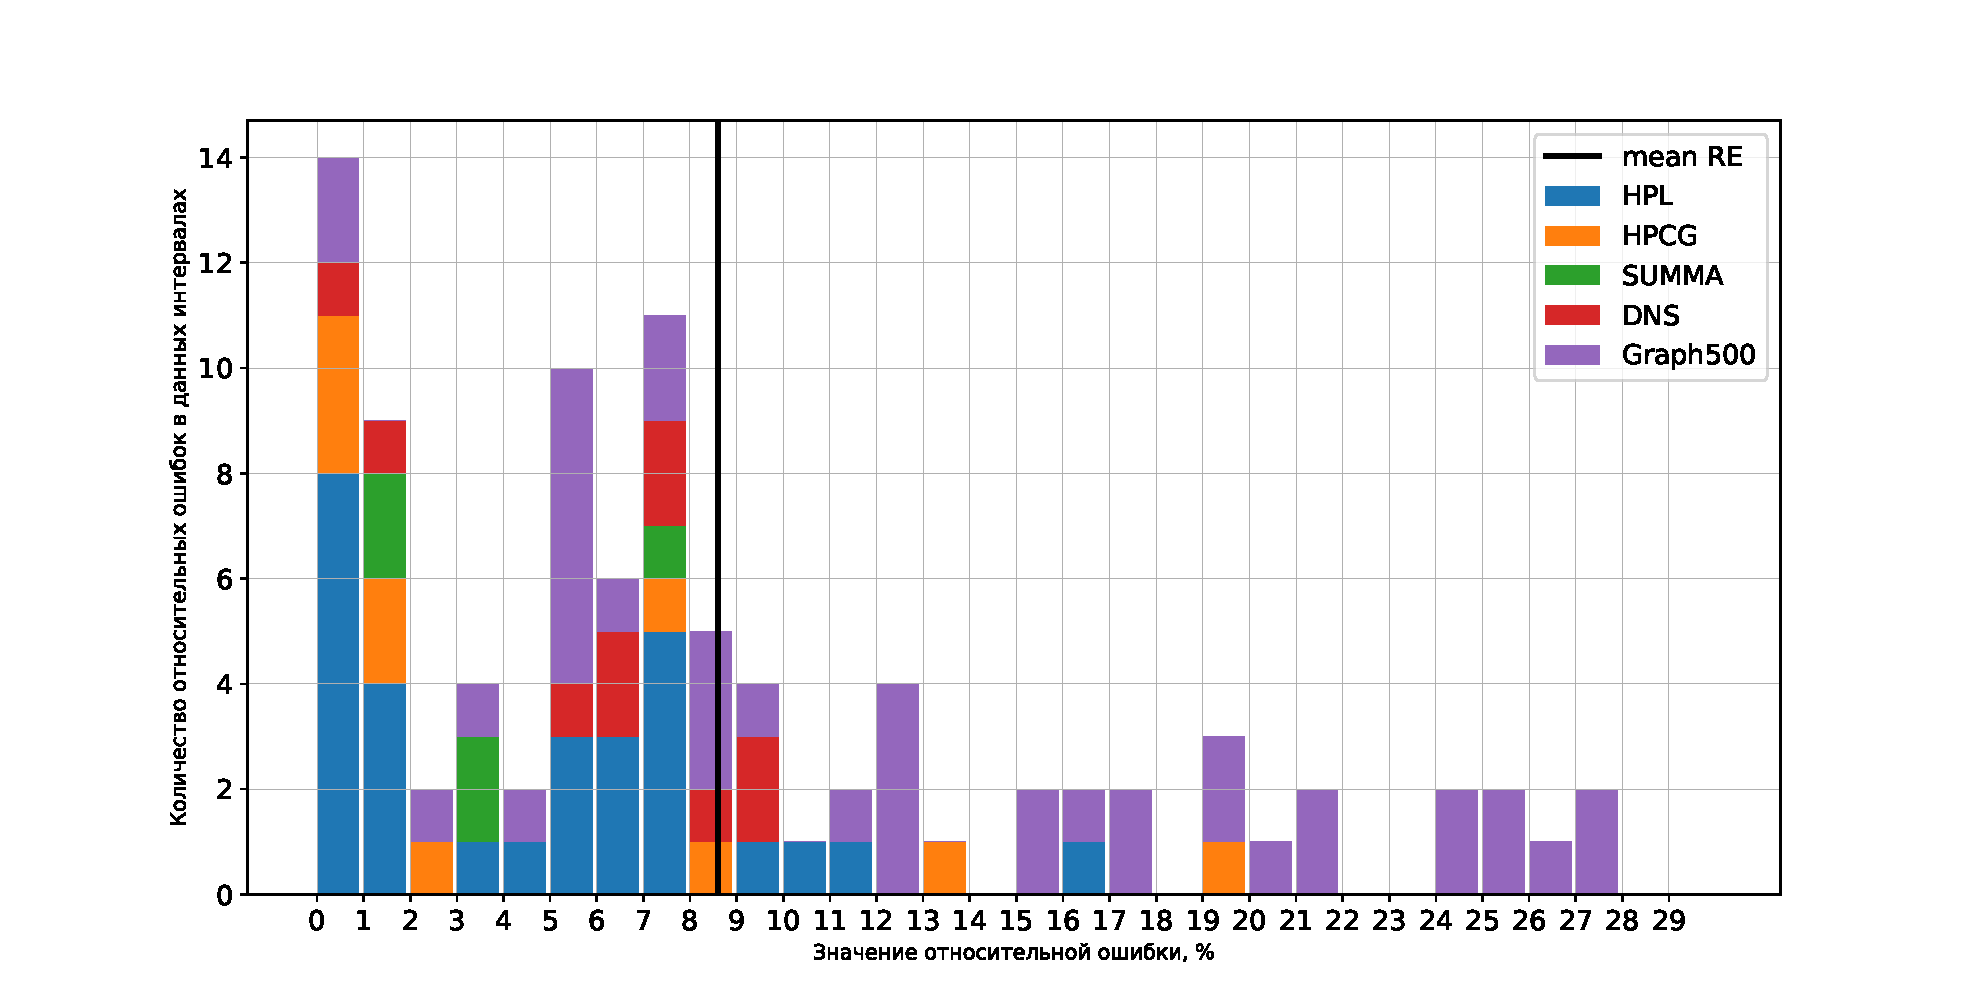
\includegraphics[width=\textwidth]{./images/RE_graph}
		\caption{Относительные ошибки предсказаний по всем рассматриваемым\newlineприложениям}
		\label{RESULT}
	\end{figure}
	В данной работе были получены следующие основные результаты:
	\begin{itemize}
		\item Разработан метод, предсказывающий слабую масштабируемость суперкомпьютерных приложений на основе экспериментальных данных со средней относительной ошибкой по всем смотренным приложениям равной 8,6\%.
		%\item Выполнена проверка применимости метода на различных приложениях, с помощью запусков приложений HPL, HPCG, матричных алгоритмов умножения SUMMA и DNS, Graph500 на суперкомпьютере "<Ломоносов-2">.
		\item Выполнена экспериментальная проверка метода с помощью запусков на суперкомпьютере "<Ломоносов-2"> на примере HPL, HPCG, алгоритмов матричного умножения (SUMMA и DNS), Graph500.
	\end{itemize}

	На основании предложенного метода удалось построить предсказания слабой масштабируемости для всех рассматриваемых приложений так, что максимальная относительная ошибка предсказания значения динамической характеристики не превышает 28\%, однако подобные ошибки, как видно, достаточно редки. Средние значения относительных ошибок для различных приложений: HPL - 4,9\%, HPCG - 5,6\%, SUMMA - 3,6\%, DNS - 6,4\%, Graph500 - 13,2\%. Средняя относительная ошибка по всем приложениям составляет 8,6\%. Гистограмма со всеми ошибками предсказаний представлена на рисунке \eqref{RESULT}. Таким образом, предложенный метод строит предсказания так, что получаемые относительные ошибки, сравнимы с ошибками предсказания у существующих подходов при сопоставимых размерах конфигураций предсказываемых запусков. Но разработанный метод отличается от них простотой построения, отсутствием необходимости собирать большой набор тестовых данных и способностью строить предсказания, не используя информацию о коде, алгоритме и системе, на которой производятся запуски, то есть он является достаточно универсальным.
	
\clearpage
%\newpage